\chapter{Automated music generation}\label{ch:automated-music-generation}

\begin{chapterabstract}
    When talking about \textit{automated music generation}, we may want to distinguish between \textit{composition assistance} (software that is not generating the music from scratch but instead helps the composer incrementally with suggestions, auto-completion, etc.) and \textit{autonomous music generation} (which takes over the whole music composing process and users are restricted just to parametrization of the generation process).
    In this chapter, we will focus on the latter.
    We will briefly go over the history of the music generation and then move on to modern techniques utilizing machine learning techniques.~\cite{music-generation-history}
\end{chapterabstract}


\section{Pre-computer techniques}\label{sec:pre-computer-techniques}

First experimentations with \textit{algorithmic composition} took place in the late 15th century by employing \textbf{"canonic composition."}~\cite{brief-history-of-algo-composition}

\textit{``The prevailing method was to write out a single voice part and to give instructions to the singers to derive the additional voices from it.
The instruction or rule by which these further parts were derived was called a canon, which means `rule' or `law.' For example, the second voice might be instructed to sing the same melody starting a certain number of beats or measures after the original;
the second voice might be an inversion of the first or it might be a retrograde [etc.]''}~\cite{history-of-western-music}

These \textit{rules} of imitation and manipulation form an \textit{algorithm} by which performers unfold the music.
In this automatical process, we see a clear removal of the composer from a large portion of the compositional process: the composer himself only invents a core of the music, a single melody or section.~\cite{brief-history-of-algo-composition}

\textit{Wolfgang Amadeus Mozart} experimented with automated composition techniques using the so-called \textit{Musikalisches Wurfelspiel} (``musical dice game'').
The game worked by joining several predefined musical segments selected by dice roll.
This simple form of \textit{stochastic} algorithmic composition left the creative decisions in the hands of chance, letting the dice roll decide what notes to use.~\cite{brief-history-of-algo-composition}


\section{Use of computers}\label{sec:use-of-computer}

There are three possible approaches when using a computer to generate a composition:
\begin{itemize}
    \item Stochastic
    \item Rule-based
    \item Artificial intelligence
    % TODO: describe the items
\end{itemize}

The \textit{stochastic} way involves \textit{randomness} and can be as simple as Mozart's \textit{Musical dice game} we already briefly touched upon;
however, we can also use more complex methods like \textit{statistical theory} and \textit{Markov chains}.
Many creative decisions are merely left to chance when generating a composition using the stochastic method.
Another example of non-computer-oriented stochastic composition can be found in Karlheinz \textit{Stockhausen's Klaveirstucke XI}, in which the sequence of various fragments of music is to be performed by a pianist in random order.~\cite{brief-history-of-algo-composition}

\subsection{Markov chains}\label{subsec:markov-chains}

So-called \textit{Markov chains} are a major technique for generating musical compositions using stochastics.
We define the Markov chain using a simple sequence of random variables $X_1, X_2, X_3, \ldots, X_i$\footnote{the index $i$ in this context is sometimes referred to as the time}; we call this sequence a \textit{stochastic process}.
For this process to be the Markov chain, the following equivalence must be true:
\[ [X_i\rvert X_1, \ldots, X_{i-1}] \sim [X_i\rvert X_{i-1}] \]
In this context, the equivalence means that the \textit{probability distribution} on the left-hand side is equivalent to the probability distribution on the right-hand side.
For a fixed value of $i$, $X_i$ is called the state of the Markov chain.
The equivalence implies that the value of $i\textsuperscript{th}$ state is purely dependent on the immediately previous state, a trait also called \textit{memoryless}.~\cite{markov-chains}

Markov chains are primarily represented in two ways a \textit{transition matrix} (figure~\ref{fig:markov-chain-matrix}) or a \textit{directed graph} (figure~\ref{fig:markov-chain-graph}).
The transition matrix $M$ is a matrix with dimensions $n$ by $n$, where $n$ is the number of different states the Markov chain maintains.
The $M_{a,b}$ value then represents $\mathcal{P}(b \rvert a)$, the probability of transition from the state $a$ to state $b$.
This representation is practical for use in computers.
The directed graph is a good representation for visualization;
each \textit{vertex} represents a state, and the \textit{directed edges} represent the probability of a transition between two states.~\cite{markov-chains}

\begin{figure}
    \centering
    \[
        \begin{blockarray}{cccc}
            & \text{Sunny}     & \text{Windy}     & \text{Rainy} \\
            \begin{block}{c(ccc)}
                \text{Sunny}     & 0.6     & 0.3     & 0.1 \\
                \text{Windy}     & 0.7     & 0       & 0.3 \\
                \text{Rainy}     & 0.5     & 0.2     & 0.3 \\
            \end{block}%
        \end{blockarray}%
    \]
    \caption{~Markov chain represented by transition matrix~\cite{markov-chains}}\label{fig:markov-chain-matrix}
\end{figure}

\begin{figure}
    \centering
    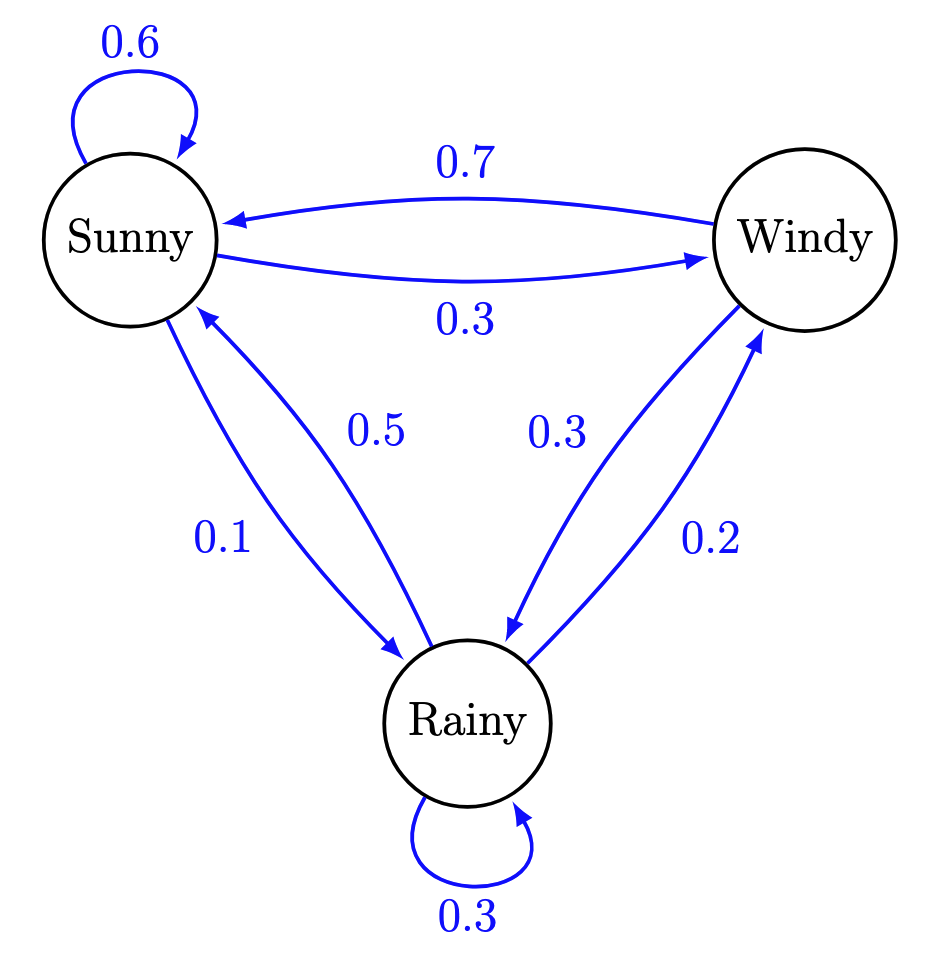
\includegraphics[width=0.5\textwidth]{assets/markov-chain-graph}
    \caption{~Markov chain represented by directed graph~\cite{markov-chains}}\label{fig:markov-chain-graph}
\end{figure}

\subsubsection{Generating music}\label{subsubsec:generating-music}

Once we have the Markov chain defined, we can use it to generate music in a simple manner;
we want to create a model that will contain sound objects (notes or chords and their duration) as states and probabilities of transitions between them.
We do this by using existing music pieces and using them as training input.
We compose the states by extracting all different sound objects occurring in the training pieces.
We can compute the transition probabilities by gathering all possible \textit{bigrams} (sequences of two adjacent objects).
The probability of transition from the state $a$ to state $b$ is then computed by following division $\mathcal{P}(b \rvert a) = \frac{\# ab}{\# ac}$, where $ab$ represents bigrams of sound object $a$ followed by sound object $b$, and $ax$ represents \textit{all bigrams} starting with the object $a$.
Using this method we compose the whole transition matrix.

With the transition matrix available, we can move on to the music generation itself.
In order to utilize the matrix for generating transitions, we first need to select the first sound object the musical piece will start with.
We can do that by manually picking the desired sound object, or we can generate it randomly by composing a vector of probabilities of starting sound objects, where the probability of each object being the starting object is the number of times it was starting object in training musical pieces divided by the total number of training musical pieces.
So to generate the piece, we select starting object from the initial vector (the likelihood of selecting an object is determined by its computed probability).
Then for every other state, we receive the vector of probabilities by using a row of the transition matrix corresponding to the current state.
We iteratively continue until we are satisfied with the length of a piece.~\cite{markov-chains}

\subsection{Rule-based music generation}\label{subsec:rule-based}

Music theory traditionally describes rules that help to direct the compositional process.
While composers regularly break those rules, they can be successfully used to implement a system for generating music.
One of the examples would be the \textit{Illiac Suite}, composed in 1957 by professors \textit{Lejaren Hiller} and \textit{Leonard Issacson}, where the rule-based system was used to help generate the first two movements.~\cite{computational-creativity}

\textit{``The general idea is to use screening rules to accept or reject randomly generated pitches and rhythms.
Probability distribution and Markov processes can also be found in the suite.''}~\cite{illiac-suite}

\subsubsection{Formal Grammars}\label{subsubsec:formal-grammars}

In the 1950s, \textit{Noam Chomsky} introduced the concept of \textit{Generative Grammars}, a tool for analyzing language that became highly influential in linguistic studies.
In a Generative Grammar, two alphabets of \textit{terminal} and \textit{non-terminal symbols} are used, along with a set of \textit{rewriting rules} given over the union of these two alphabets that allow transforming non-terminal symbols (or string of non-terminal and terminal symbols) into other symbols (both terminals and non-terminals).
The generated \textit{language} is the set of all possible strings of terminal symbols generated from a special starting variable (usually called $S$) and applying any number of rewriting rules in sequence.
These Grammars can be seen as an implementation of the beforementioned rule-based systems.~\cite{computational-creativity}

\textit{Lindenmayer Systems} (L-Systems) are a variant of Generative Grammars used for music generation;
the difference from Chomsky's Grammars is that they implement \textit{parallel rewriting}, applying all the rewriting rules at once instead of only one at a time.
This characteristic makes these systems less inclined to generate sequential data, like simple melodies, and have been used to generate stunning visual effects.
When applied to music generation, a common approach was to map visual data generated by \textit{L-systems} to score information or to a sequence of musical segments.~\cite{computational-creativity}

One of the most influential researchers of rule-based music generation is \textit{Ebcioǧlu}, who implemented a custom logic language that he used to create \textsl{CHORAL}, a system for the generation of Bach-like chorales that uses some 350 rules for harmonization and generation of melodies~\cite{ebcioglu}.
The hardship of designing such a system lies in the complexity of explicitly coding enough rules, many of which often do not have a formal definition in musicology literature.~\cite{computational-creativity}

\subsection{Artificial intelligence}\label{subsec:artificial-intelligence-music-generation}

\textit{``Artificial Intelligence (AI) is the property of machines, computer programs and systems to perform the intellectual and creative functions of a person, independently find ways to solve problems, be able to draw conclusions and make decisions.''}~\cite{about-ai}

AI is a buzzword that contains two main branches, the original \textit{symbolic AI} and \textit{machine learning}.
The symbolic AI are systems where we capture knowledge using formal mathematical logic, genetic algorithms, state-space search, automated planning,~\ldots~.
The machine learning AI builds models with a set of hidden internal parameters we are trying to fine-tune so that the model performs well on predefined metrics;
this optimization process is called learning.
In this thesis, we will specifically focus on \textit{artificial neural networks}, which are subset of ML techniques.

The increased computational power of computers and the widespread general-purpose GPU programming recently made \textit{deep learning}\footnote{use of ANNs with more than three hidden layers} techniques extremely popular, with applications spanning from \textit{NLP} to \textit{image processing} to \textit{music generation}.

While the interest in these algorithms grew exponentially in the last decade, the first music generation system to use ANNs was that of Peter M. Todd\cite{first-ann-mgs}, who used a three-layered \textit{Recurrent Neural Network} (RNN) to generate monophonic melodies.
Recurrent Networks reuse the results of the computations from previous steps every time a new input is fed, allowing them to encode temporal sequences.
Still, standard feed-forward networks are also an option for music generation.
There is also room for standard feed-forward networks: in 1991, J. P. Lewis trained a network\cite{feed-forward-ann-mgs} with musical patterns ranging from random to well-constructed to learn a measure of ``musicality'' used by his music generation system to select pleasing compositions.

As mentioned, RNNs are a popular choice for music generation.
In particular, \textit{LSTMs}\cite{LSTMs} are a special variant of recurrent networks that use gates to decide the amount of information taken from novel input and what is maintained from older inputs, hence the memory.
The first LSTM used for music generation was applied to blues improvisation\cite{LSTM-mgs}.
Another deep learning approach is that of Generative Adversarial Networks (GANs)\cite{gans};
the concept behind this method is to train two networks at the same time, one generates musical compositions imitating what is learned from real-world examples, and the other tries to discriminate between original and imitated compositions.
As one network gets better, the other must improve as well in order to ``beat'' the other network (therefore making them ``Adversarial'').

